\chapter{Design} \label{design}
In this chapter we focus on the prototype VR application which is implemented. Before starting with the development, the content of the application has to be set. Also the requirements of the application have to be clear. For which target group the application is developed? What is the storyline of the application? How will the application be used later on? In the following, we shortly introduce, what kind of process model we choose for the implementation. After that, we set the requirements and target group for the prototype. The application will have a fictive storyline, similar to a computer game. In order to design the story, we create a storyboard and present it in this chapter. Once the content is set, we take a look at designing a dialogue with the user and choose suitable user input methods.
\section{Process model}
The objective of this thesis is to develop and evaluate a prototype VR application to simulate the different IT courses offered at NYP. To handle a complex task like this, it is important to apply a suitable process model. The project is developed in a group of two people, therefore a model like SCRUM would not be suitable in this case. Nevertheless, we divided our project in iterations and did a review after the end of each iteration. For this project an iteration of six weeks is chosen. The review contains a presentation in front of the supervisor and two independent lecturers. They give feedback about the prototype and ideas for enhancement. Every week, there is a meeting with the supervisor, in which current problems are discussed and tasks are set. For organizing our tasks we use elements from the process model Kanban, because this model helps keeping an overview of the status and the progress of different tasks. We visualise the tasks as cards and display them on a board, which can be seen in  figure \ref{fig:board}. Each card has a description, an assignee and an importance level. The cards are put in different containers: To-do, in progress, ready for testing and done.\\
Each IT course, which is planned to be represented in the VR application will be treated separately. This means, that during an iteration, not more than one job role will be in focus of the design and development part.  
\begin{figure}[h!]
  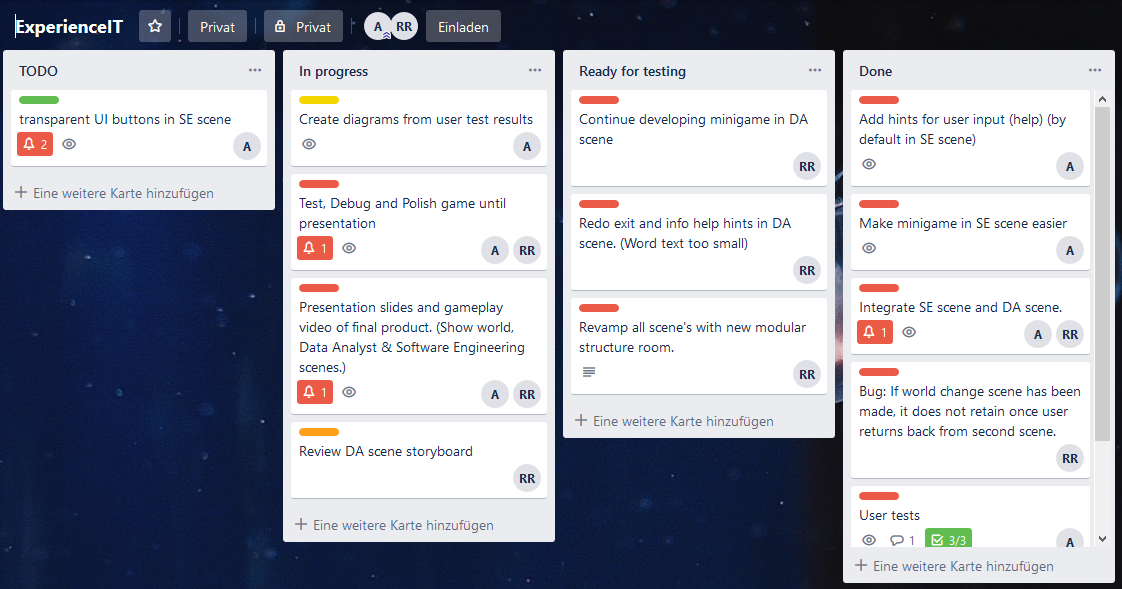
\includegraphics[width=16cm]{kapitel/kanban-board.png}
  \centering
  \caption{Board for visualising tasks and workflow.}
  \label{fig:board}
\end{figure}
\newpage
\section{Requirements}
In order to achieve the main objective of this work, several functional requirements have to be set:\\
\begin{itemize}
\item Introduction: The application should introduce the user to the various IT job roles.
\item Start scene: The application starts in a futuristic city which can be explored by the user.
\item Interaction: The user can interact with several objects in the starting scene and enter different scenes through this.
\item Separation: Each job role should be presented in a separate scene. The user should be aware of which job role the scene is referring to at all times.
\item Completing tasks: Each introduction of a job role should contain information of the job and a task which should be completed by the user.
\item Main storyline: There should be a main objective and each job role task is a step towards completing the main objective.
\item Gamification: The tasks should be structured as minigames and there should be a reward after completing them successfully.

\end{itemize}
Besides the functional requirements, there are several non-functional requirements which have to be considered when developing the prototype:
\begin{itemize}
\item Interesting: The user should gain more interest in the job roles introduced in the VR prototype.
\item Setting: The application should take place in a futuristic environment. Users should see how they can impact the future with IT.
\item Genre: The application should be a mix between a informative educational and a gaming application.
\item Educational: The user should gain more knowledge of the IT job roles after playing the VR application.
\item Portable: The application should be presented at various public events, such as open houses or fairs.
\item Budget: The product will not be distributed commercially. Therefore the costs for external tools, graphic or audio assets should be held to a minimum.
\end{itemize}

\section{Stakeholders}
In this chapter we define actors for the VR application. This is done by naming the different stakeholders of the application.
Stakeholders have different interests and expectations to the project. The \textbf{School of Information Technology} would like to have more students signing up for an IT course. They expect that the VR application arouses interest in IT by prospective students. Their task is to provide the application at public events, such as open houses and similar events. The School of Information Technology is also responsible for providing the IT courses which are introduced in the VR application. \\
The \textbf{project leader} expects a structured and well communicated application development. They expect that the objectives of the work is clear and the deadlines are met. The project leader is responsible for the guidance of the developers and the communication between the customer (School of IT) and the developers. The project leader sets and monitors the milestones in collaboration with the developers.\\
The \textbf{prospective students} are the end users of the VR application. They expect a joyful experience while using the application. They also want to learn more about the IT courses offered at NYP. Their task is to play the actual application. In case they are interested in one of the IT courses, they are responsible in applying for a diploma course at NYP.\\
The \textbf{developers} expect clear objectives from the project leader and a detailed description of the requirements. Their responsibility is to provide the actual application based on the frame given by the project leader and the customer. They develop a storyline, program the application and test it as well. In close communication with the project leader, they apply changes to the system.
\section{Target group}
Before starting with the design of the application, we have to define the target group. This makes developing of the application purpose easier and also helps keep the focus during the design process. A very important aspect of defining a target group is also, to develop the application directly to the needs of the future users. In the end this helps to increase the acceptance of the application. 

The main target group of the VR application will be prospective students, who are considering to sing up for a diploma course at NYP. As mentioned in the introduction, those students mostly come from a secondary school and have finished their O-Levels, which is an entry requirement for polytechnics. The secondary school educated the students on a very widespread basis, and the students can now decide their specialisation. \\
When the students leave their secondary school, the average age is 16. At this age, people are known to be open to new technologies and trends. The people in the target group are in the stage to make independent decisions for themselves without influence of parents. The application will be designed for prospective student which show an interest in information technology but yet have no experience or knowledge in that field.\\
In the following, a characteristic of a fictive person is displayed. This person stands as a representative for the target group of prospective students:

\paragraph{Characteristics}
\begin{description}
	\item[Name:] Jessica Lee
	\item[Age:] 16
	\item[Place of residence:] Singapore
	\item[Education:] Finished secondary school
	\item[Personal interests:] Dancing, computer games, TV series, technology
	\item[Level of tech experience:] Rich consumer, no programming skills
	\item[Expectation:] Wants to experience a fun virtual reality application
\end{description}
Since the fictive person Jessica Lee's main expectation is to experience a joyful application, there will be the need of gamification elements in the application. Her interests in computer games and technology lead the application's scene setting into a futuristic environment with new technologies. She has experience in digital media as a consumer, but not as a professional. Therefore, common gestures for user interaction can be applied, but the difficulty level of tasks about information technology should be on a beginner level. 
\section{Main story concept}
To gain the users attention and let them grow interest in the application it is important to have a good main story. The main story will create a bridge between the several IT courses displayed in the application. The story we present in this chapter is the main story line of the final product. We will only be able to realize parts of the main story in this work.\\
The VR application, hereinafter called game, will start in the so called ``Smart City''. This is a futuristic urban environment in which the user can move around freely. There are five different buildings along the streets. Each building is interactive and represents a course offered by NYP. When interacting with the buildings the user can enter laboratories, so called ``labs'', and complete different tasks. Every successful completion of a task has an impact to the main story. \\
The main goal of the game is to create a delivery drone which will deliver orders from online shops. This is still a vision of future for now, but it is a good showcase for the user to show them how they can impact the future with IT. During the completion of the labs several challenges will occur. Once the user started programming their first drone, a lot more drones will start flying around in Smart City. To avoid crashing and chaos, the next task is to provide a proper and stable internet connection to the drones, so they can communicate. But the connected drones have their advantages and disadvantages: At first they are flying normally and communicating to each other but then an unknown IoT-Hacker infiltrates a virus into the drone firmware, so they start to misbehave. Now the user has to trace the hacker with basic cyber security concepts. After the hacker was found, more and more inhabitants of Smart City start to use the drones and provide a lot of data. It is now the job of the user to analyse this data and optimise the drones. By combining relevant data, it is possible to add some enhancements to the drone.
Once the user completed all tasks and visited all labs, the user can exit the game. \\
During the development process of this work, it will not be possible to implement the whole main story and add all job roles. Instead, we will concentrate on one or two job roles. Other job professions will be added in an iterative process.
\newpage
\section{Storyboard}
In this chapter, we explain the structure and the details of the main storyline with the use of a storyboard. Since the requirements for the prototype application are already set, the storyboard points out the details of the requirements in a visual way.
The main objective of a storyboard is to get a scene by scene overview of the story and the sequence of events. Through a sketch draft, an idea of the visuals of the application is displayed. The focus of the storyboard lies on the storyline. Logical orders of scenes are displayed with arrows, textual explanations are added whenever necessary.\\
For the storyboard of the prototype, a tool called \textit{Invision freehand}\footnote{\label{foot:2} \url{https://www.invisionapp.com/feature/freehand}} is used. In the following, some important parts of the storyboard are presented \footnote{\label{foot:3} The complete storyboard can be seen in: \url{https://www.invisionapp.com/feature/freehandhttps://projects.invisionapp.com/freehand/document/Vbu2DFCdd}}. We introduced the IT courses from NYP in chapter
\ref{stateofart}. The final product should contain all job roles of the courses, but for the prototype in this work we focus our design on the job role of the software engineer scene and the cyber security specialist scene.
\subsection{World scene and software engineer scene}
\begin{figure}[h!]
  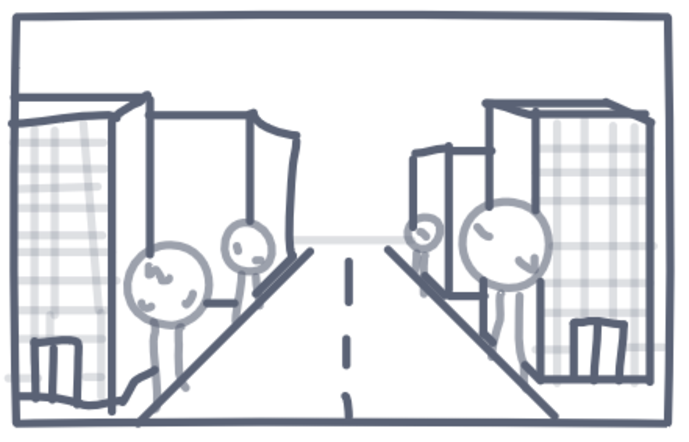
\includegraphics[width=8cm]{kapitel/storyboard/smart-city.pdf}
  \centering
  \caption{Smart city scene from where the user can explore different IT job roles (own illustration)}
  \label{fig:smartcity}
\end{figure}
The first scene of the storyboard is the smart city scene, as sketched in figure \ref{fig:smartcity}. Here the user can walk around freely. When the user selects the software engineer building, an assistant asks the user to enter the building. If the answer is ``yes", there is a transition into the software engineer lab scene. The lab contains a testing drone and a package as well as working desks with laptops. After the transition, the assistant explains the first task, as displayed in figure \ref{fig:sescene}. This is the first minigame, in which the user should gain understanding in how programming works.
\begin{figure}[h!]
  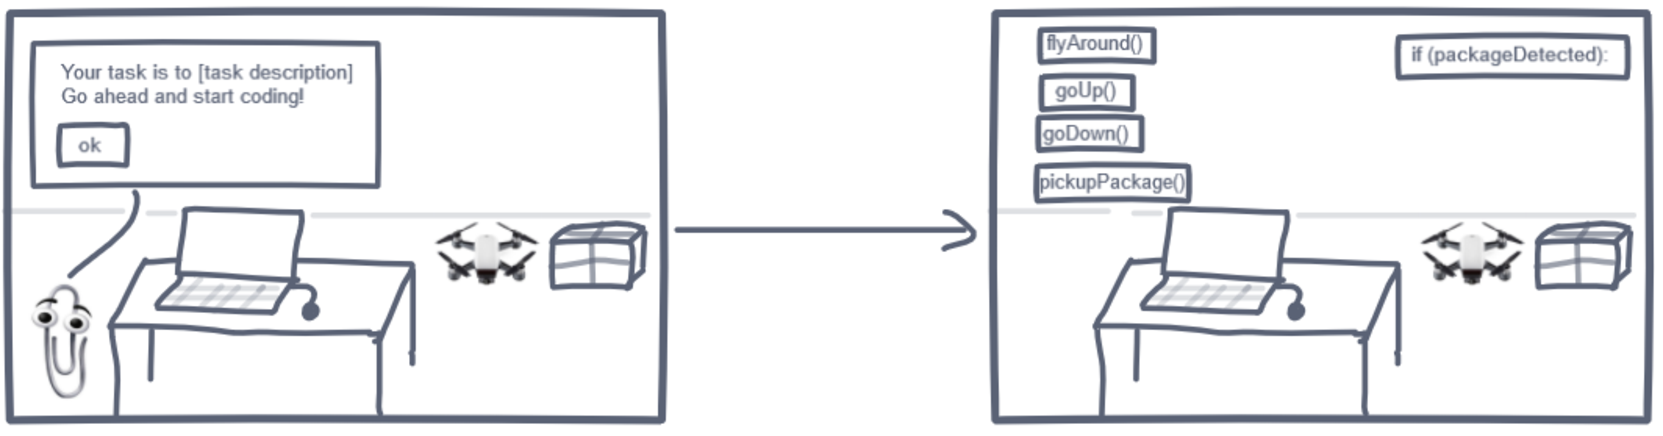
\includegraphics[width=16cm]{kapitel/storyboard/se-scene.pdf}
  \centering
  \caption{Software engineer scene: dialog and minigame (own illustration)}
  \label{fig:sescene}
\end{figure}
\\The information is taught in a very simplfied way, because the requirements of the application are that it should be playable without knowledge in IT. The objective of the task is to program the package delivery drone, so that it actually picks up a package. This is done by arranging lines of code in a logical order. The working environment is a desk with a laptop. After the user has arranged the code blocks and ran the code successfully, they can watch the testing drone in the lab picking up the package. With the completion of this minigame, the scene ends and the user is transferred back to the world scene.
\subsection{Cyber security specialist scene} 
The second scene represents the job role of the cyber security specialist. The scene is a laboratory with several office working places and the drone from the previous scene which is displayed on a table in the middle of the room. When the user enters the lab, they are informed that the drone they had programmed before was corrupted by an unknown hacker. During the next task, the user should gain knowledge in the methods cyber security specialists use to investigate digital crimes. The user learns about simple data decoding and encoding as well. The minigame is divided into three parts. 
\begin{figure}[h!]
  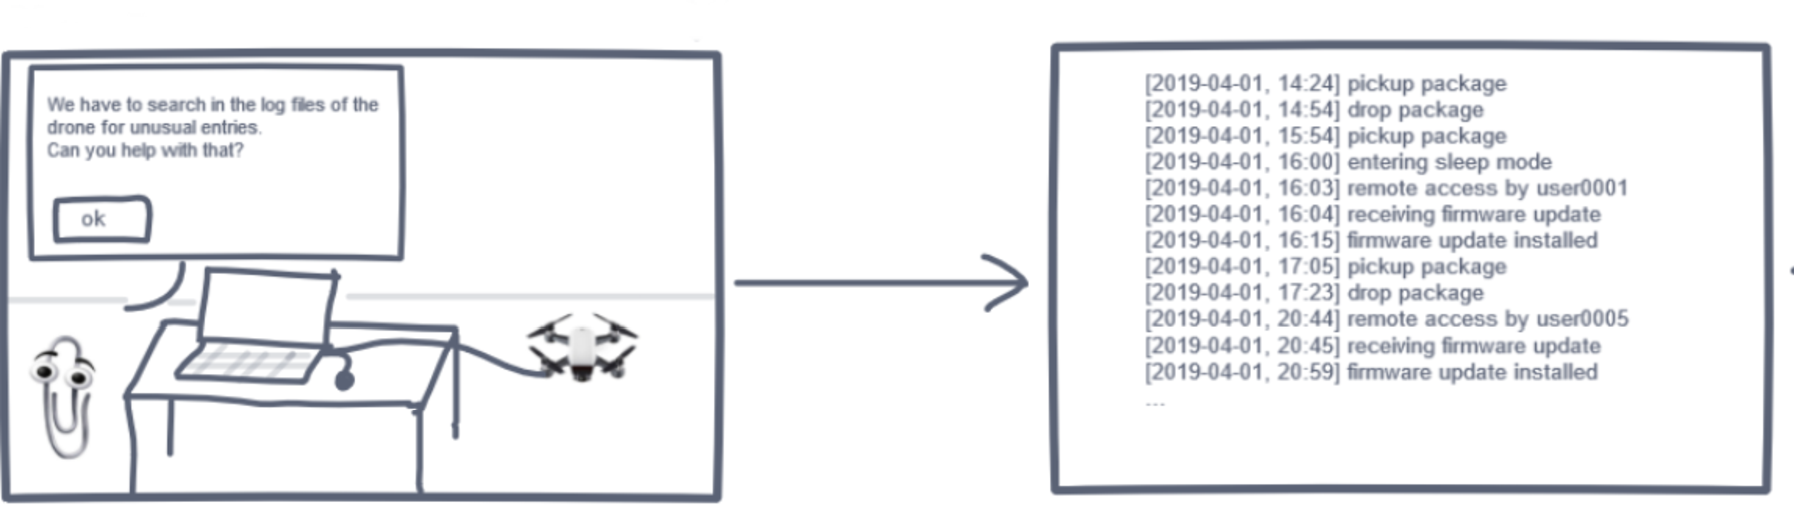
\includegraphics[width=16cm]{kapitel/storyboard/cyber-analyst1.pdf}
  \centering
  \caption{Cyber security specialist scene: searching log entries (own illustration)}
  \label{fig:logscene}
\end{figure}
\\In the first part, the user searches the log data of the drone for unauthorized access and marks suspicious entries which can be seen in figure \ref{fig:logscene}. It turned out that two lab employees have accessed the drone during the last 24 hours. in the second part of the minigame, users search the computers of the two lab employees for further information. 
\begin{figure}[h!]
  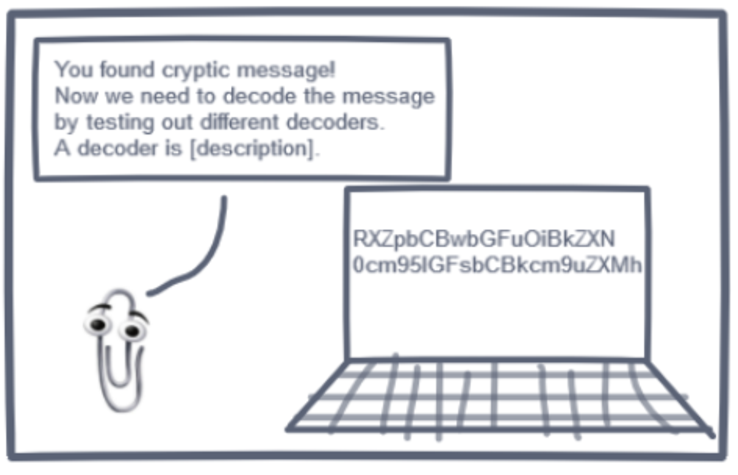
\includegraphics[width=8cm]{kapitel/storyboard/cyber-analyst3.pdf}
  \centering
  \caption{Cyber security specialist scene: encrypted message}
  \label{fig:logscene2}
\end{figure}
One employee has an encoded message on their desktop (figure \ref{fig:logscene2}).\\ Finally, in the last section, users decode the message by trying out different commonly used codes. The message reveals the hacker and the person can be prosecuted. This marks the end of the cyber security specialist scene.

%\section{Hardware evaluation}
%Looking at the requirements, one of the constraints for the application is, that it should be portable. Another requirement is, that the budget should be held to a minimum. This limits the number of hardware devices, which can be used within the VR application. When it comes to choosing a HMD, there is the decision between mobile HMD and desktop HMD. Since a mobile HMD fulfills the requirement of portability better than the dektop linked version, this is the preferred HMD.\\
\section{Dialogue design}
As seen in the storyboard, the application contains a lot of conversation between the assistant and the user. The dialogues are very important for the game, because they provide all the relevant information about the IT job roles. The dialogues should be presented in a natural and interesting way, because the application should arouse interest in IT job roles.\\
Spoken dialogue systems are the most natural way of communication, but on the other hand they are not easy to realise and need a lot of computation. This application will therefore stick with a text based dialogue system. To still provide a natural experience to the user, the dialogues should be mixed with interactions. Nevertheless, a voice over will be considered for the final product, but not for this prototype. \\
\begin{figure}[h!]
  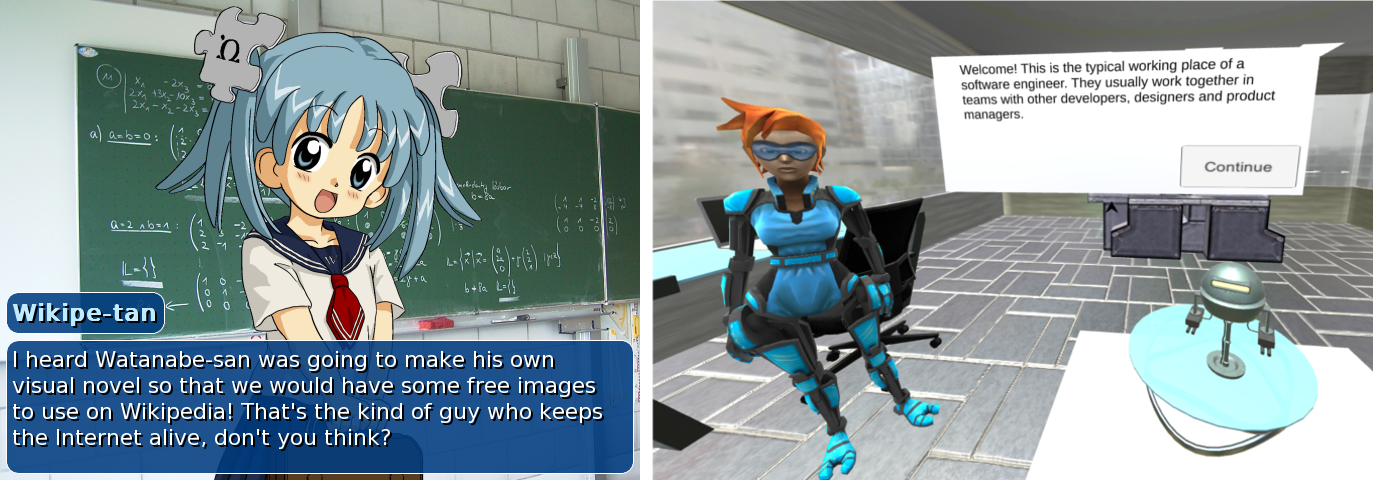
\includegraphics[width=16cm]{kapitel/screen-vs-world-dialog.png}
  \centering
  \caption{Screen space dialogue panel by \cite{screenspace} vs. world space dialogue panel.}
  \label{fig:screen-world-dialogs}
\end{figure}
When it comes to displaying the dialogue text in VR, there are some differences compared to a 2D space text displaying method. In 2D interfaces, for example in computer games, the conversation text of non playable characters (NPCs) is often displayed on the bottom of the screen and fixed to the screen space, like it is displayed in the left picture of figure \ref{fig:screen-world-dialogs}. This cannot be realised in the same way in VR. Users are not able to focus a screen space text when it is not directly in the middle of their view. Therefore, the dialogue texts are placed into the virtual world space, like seen in the right picture of figure \ref{fig:screen-world-dialogs}. The challenge of this method is to guide users to the position, where the dialogue is displayed. This is realised by placing the dialogue panel close to interactive items in the game. Once the user interacts with the items, the dialogue starts. The user is already focusing the objects and will notice the dialogue appearing in their view. Another method is used when there is a dialogue at the beginning of a new scene: The user's position and view is set close to the dialogue panel initially.
\section{User interactions}
In chapter \ref{stateofarts} we already introduced the different user interaction methods in VR that are commonly used. In this chapter we take a look at the different methods and evaluate, which method is the most suitable for the prototype VR application. There are several constraints and limitations in user interaction because of the hardware and the budget for the project. User interactions should also fit to commonly known user interactions like touch gestures or first person walking in computer games.\\
First of all we have to evaluate, what kind of user input Samsung Gear VR as well as Oculus Go provide out of the box.
The following input methods are available with the Samsung Gear VR: A wireless handheld controller or a touchpad attached to the HMD. Oculus Go provides a handheld controller which works the same way as the controller of Gear VR, but no touchpad at the HMD.\\
\begin{figure}[h!]
  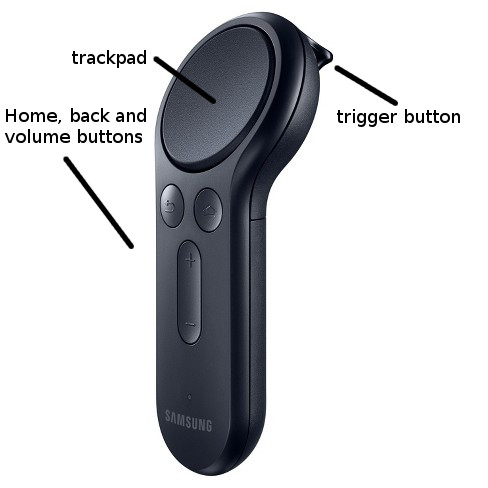
\includegraphics[width=10cm]{kapitel/samsung-controller.jpg}
  \centering
  \caption{Samsung Gear VR handheld controller \cite{Samsung.2019b}}
  \label{fig:samsung-controller}
\end{figure}
The handheld controller has gyro-sensors to detect its rotation but there is no position tracking. This means that the current controller  position is not mapped into the virutal world. As a workaround it is possible to reset the positioning of the controller with a button click.
The controller can either be used with the left or right hand. In order to use the controller, it has to be connected with the phone via bluetooth. To register user input, there are several buttons/trackpads, which are described in figure \ref{fig:samsung-controller}. The trigger button is a primary button, which can be pressed with the index finger. There is a trackpad which registers the thumb position and has a primary button as well. The last primary button is the back button. The controller registers the hand or arm rotation through sensors. There are home buttons and the volume buttons which are reserved by the system. The handheld controller of Oculus Go has the same buttons and functionalities, except the volume buttons which are located at the HMD directly.\\
The touchpad, located on the side of the HMD from Samsung Gear VR, registers touch position and touch gestures. Unlike the handheld controller, the touchpad does not need to be connected manually and always registers user input, when the HMD is used. It is therefore often used as a backup solution, in case no bluetooth controller is connected. However, the touchpad is only available for the Samsung Gear VR. We want the application to work with Oculus Go as well as with Samsung Gear VR. Therefore, the user input development is focused on the usage of the handheld controller.\\
Looking at the story board, several user interactions can be extracted:
\begin{itemize}
\item Relocating in the virtual world
\item Selection of objects
\item Relocating objects
\item Dialogue between assistant and user
\end{itemize}
First of all, we take a look at relocating in the virtual world, which is walking in VR in other words. Natural walking methods cannot be used because of missing hardware sensors. With the use of the handheld controller, the teleporting method or the camera manipulation method can be used. Since the target group are secondary students which are experienced in the usage of digital media, the method of the camera manipulation is chosen. It is expected, that the target group is already introduced to this kind of relocating, since it is widely used in computer games. To reduce the risk of motion sickness, the walking speed is held slow. The user can start walking when pressing the index trigger button. The direction of walking can be changed by moving the head.\\
The selection of objects is done with the help of the handheld controller. When using a controller, the ray-casting method is a very straightforward method for selecting. Ray-casting is also used in the default home application from Oculus. It is better to reuse well established user interface concepts than to introduce new input methods. Therefore, the ray-casting method is chosen for selecting objects in the VR prototype application. The implementation will be similar to the Oculus home application.\\
Relocating of objects is necessary when completing tasks. Especially during the minigame in the software engineer scene where the user has to arrange lines of code in order to code the software for the drone. To relocate the lines of code, the drag and drop method is chosen. By pointing and clicking on an object, it starts to follow the controller movements. Clicking again, the current position is applied to the object and its position is fixed in the world space. This is similar to a drag and drop action on 2D interfaces. Every object which has an interaction, will be highlighted when the user points with the controller at it.\\
The dialogue between user and the assistant is solved via a text based dialogue system, which is used in retro games for example. The user can control the dialogue flow and answer questions through simple button clicks.
